

\section{Phonon heat transfer}


\subsection{Energy transfer through a constriction (Publications \cp{fpu}, \cp{fpu2}, \cp{gf})} 


\begin{figure}
\begin{center}
 %\includegraphics[width=8.6cm]{../scbaths_paper_re_resubmission/pic1.ps}
 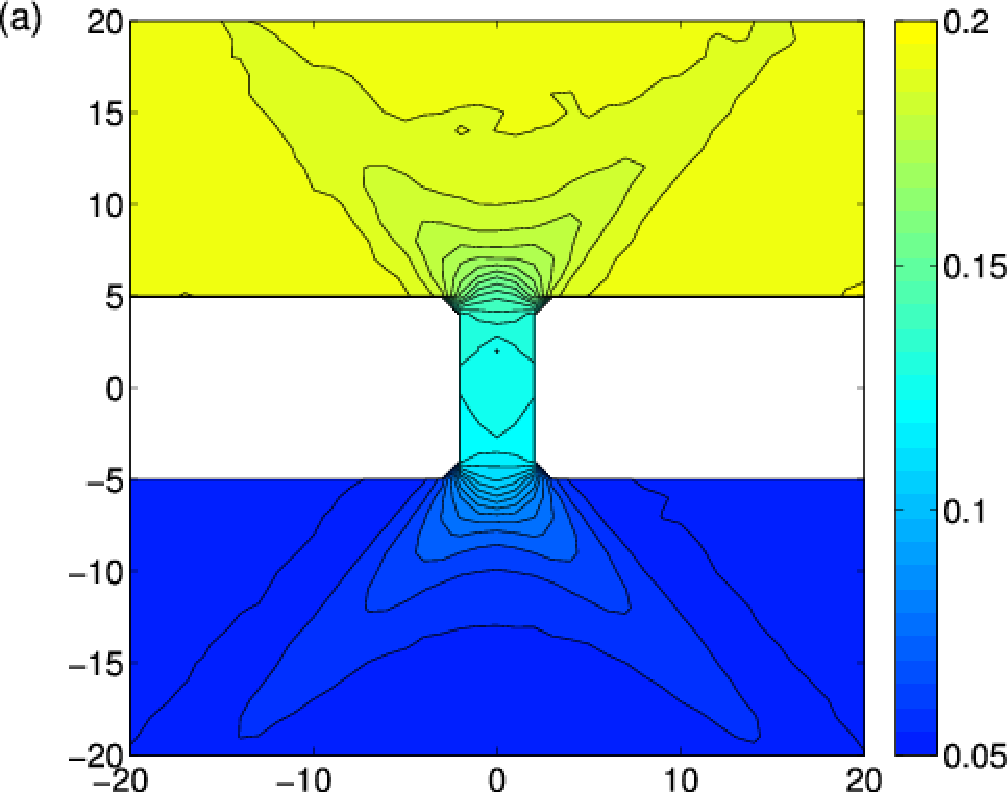
\includegraphics[width=.49\columnwidth]{pics/fpu_fig2a.pdf}
  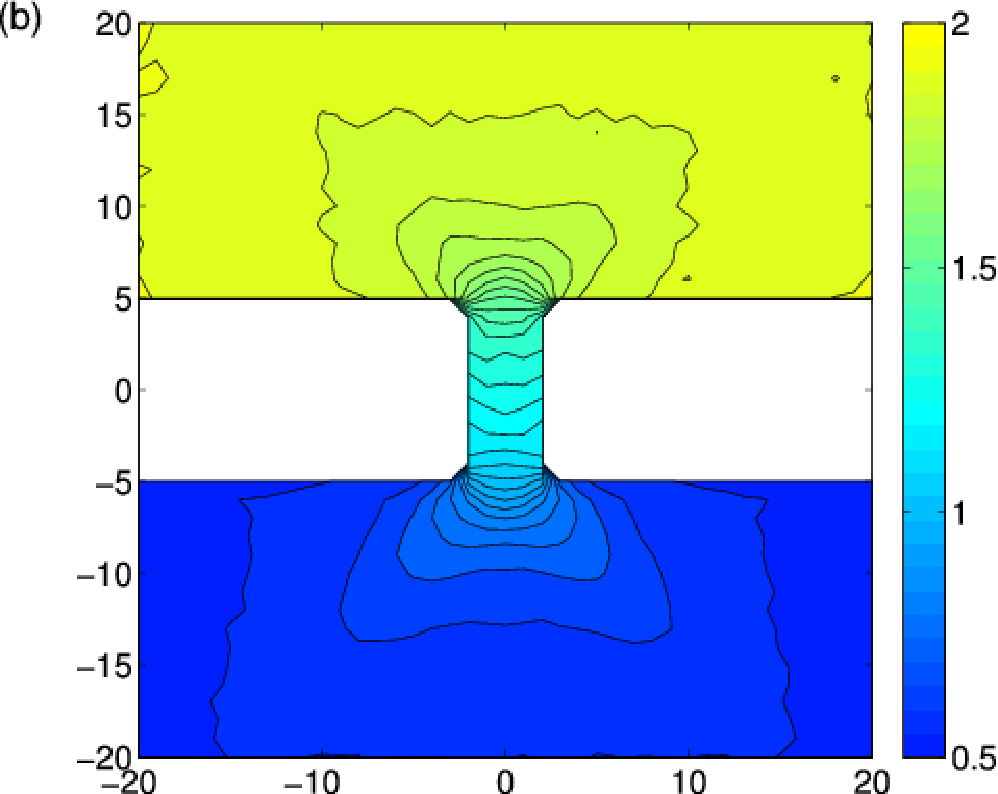
\includegraphics[width=.49\columnwidth]{pics/fpu_fig2b.pdf}
 \caption{Kinetic temperature profile at (a) low temperature ($T_+=0.20$, $T_-=0.05$) and (b) high temperature ($T_+=2.0$, $T_-=0.5$). The bulk size is $W^R=161$, $L^R=80$ and the constriction size $W^C=5$, $L^C=9$. The labels on the horizontal and vertical axes mark the atom indices. The separations of isolines are (a) $0.005$ and (b) $0.05$.}
\label{fig:fpu_fig2}
\end{center}
\end{figure}

\begin{figure}
\begin{center}
 %\includegraphics[width=8.6cm]{../scbaths_paper_re_resubmission/pic1.ps}
 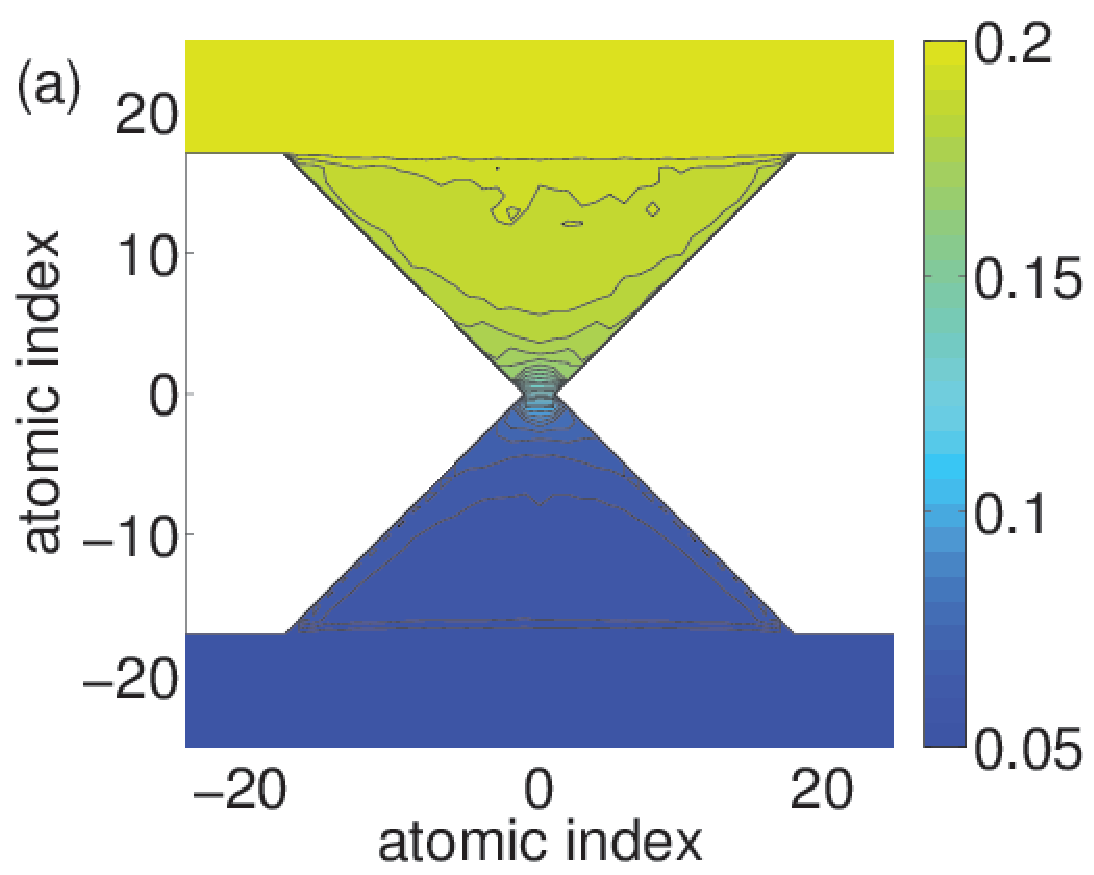
\includegraphics[width=.49\columnwidth]{pics/aip_fig5a.pdf}
 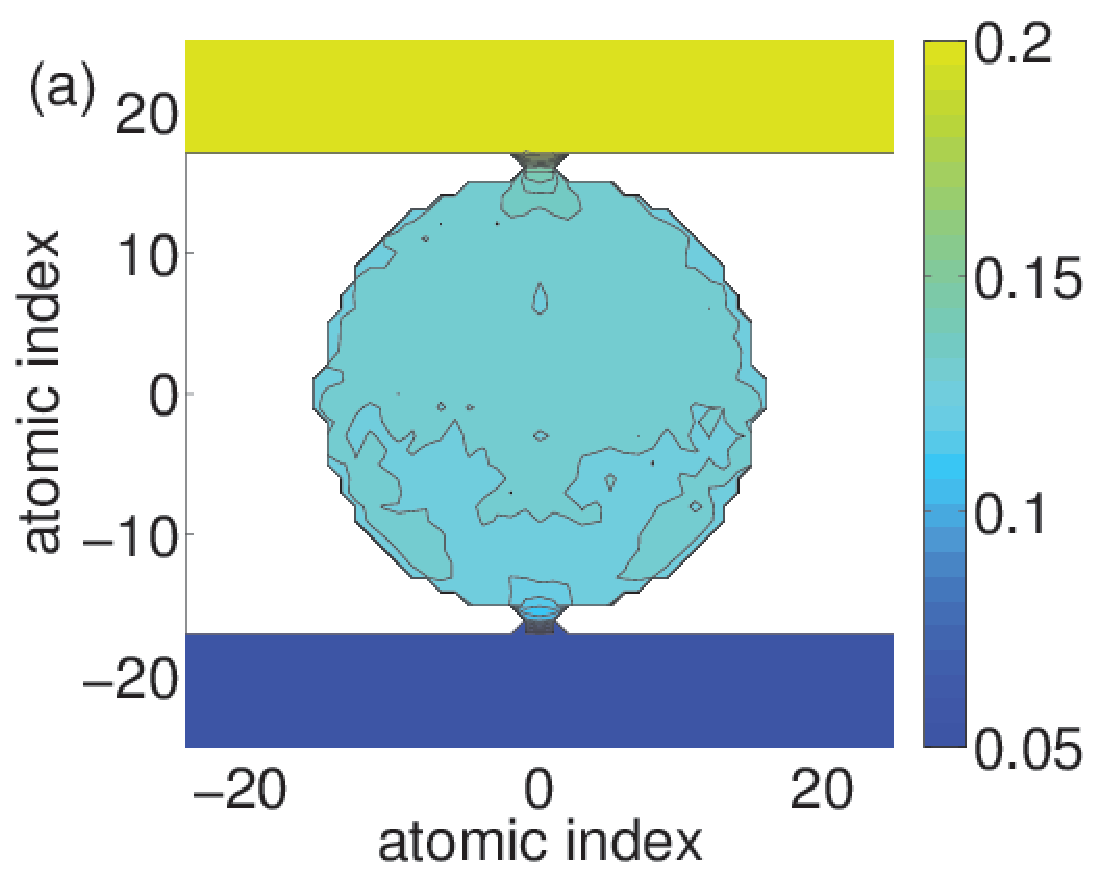
\includegraphics[width=.49\columnwidth]{pics/aip_fig6a.pdf}
 %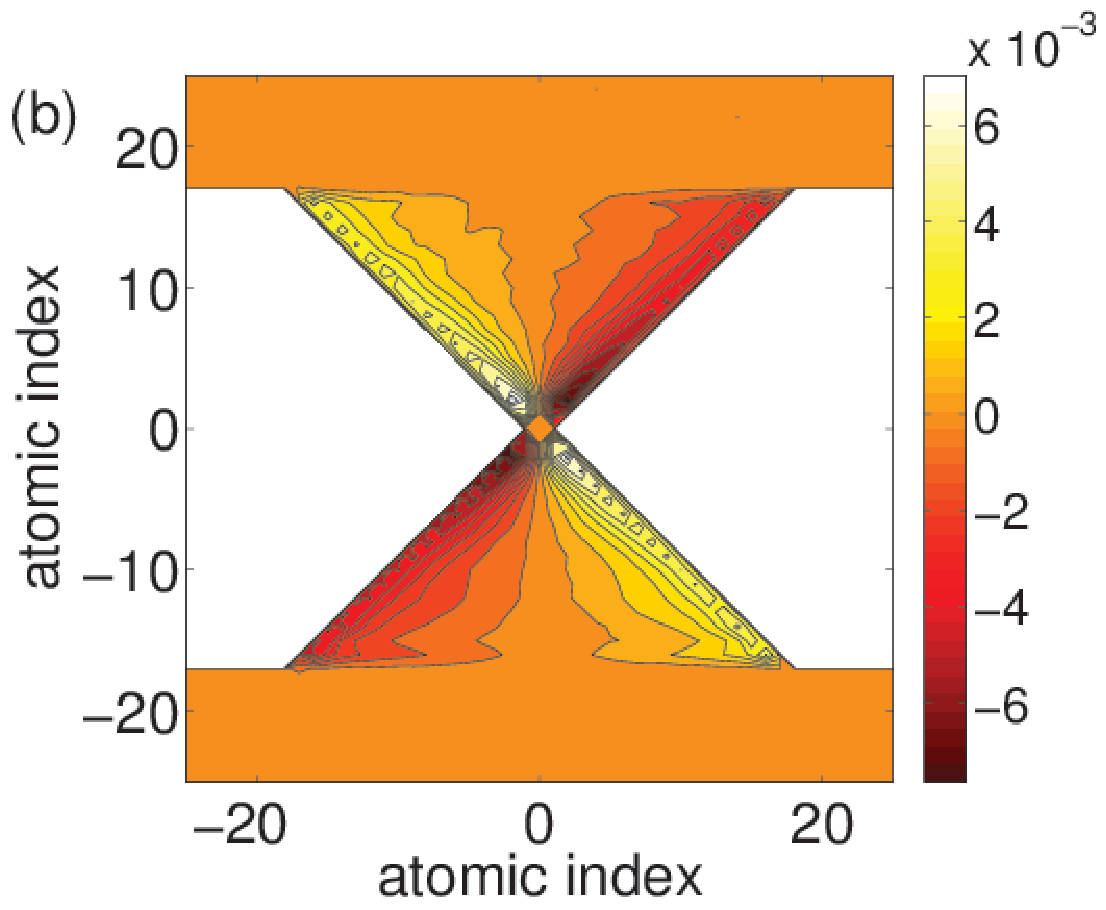
\includegraphics[width=.49\columnwidth]{pics/aip_fig5b.pdf}
 \caption{Kinetic temperature profile in (a) triangular constriction (b) discoid constriction. The separations of isolines are (a) and (b) .}
\label{fig:aip_figs56}
\end{center}
\end{figure}

\begin{figure}
 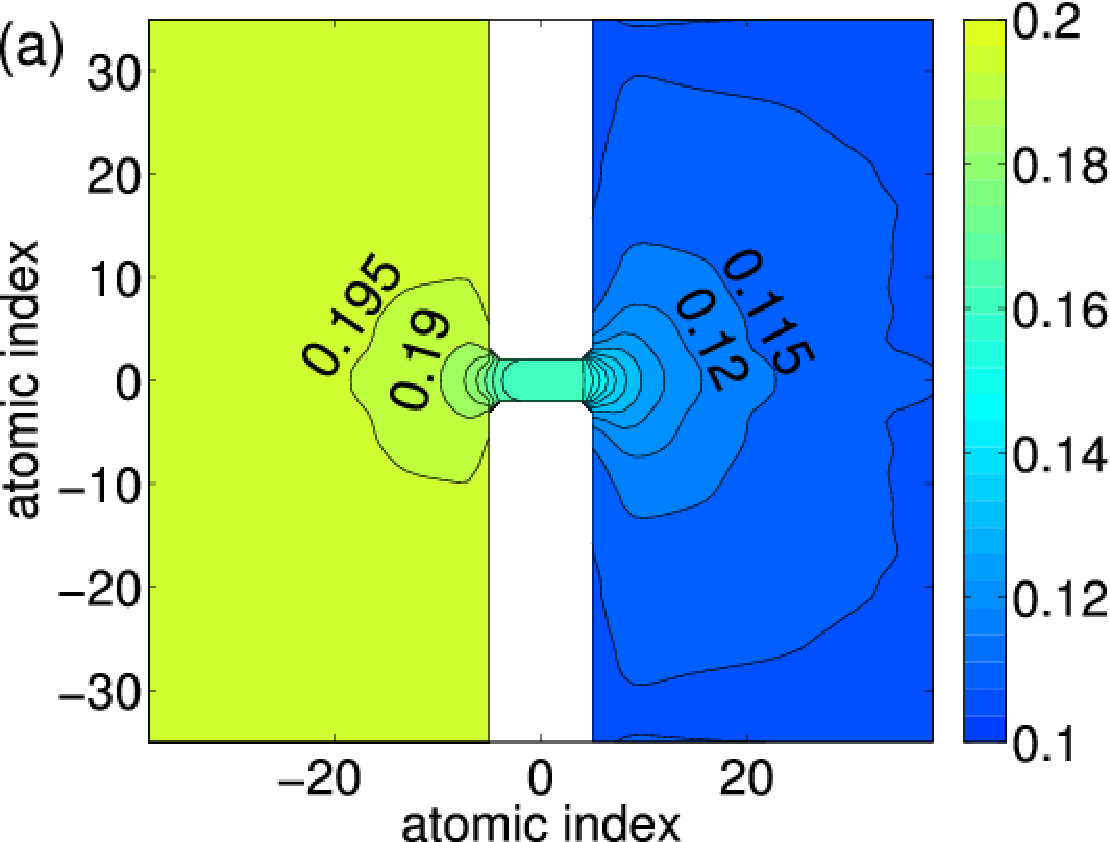
\includegraphics[width=.49\columnwidth]{pics/gf_fig7a.pdf}
 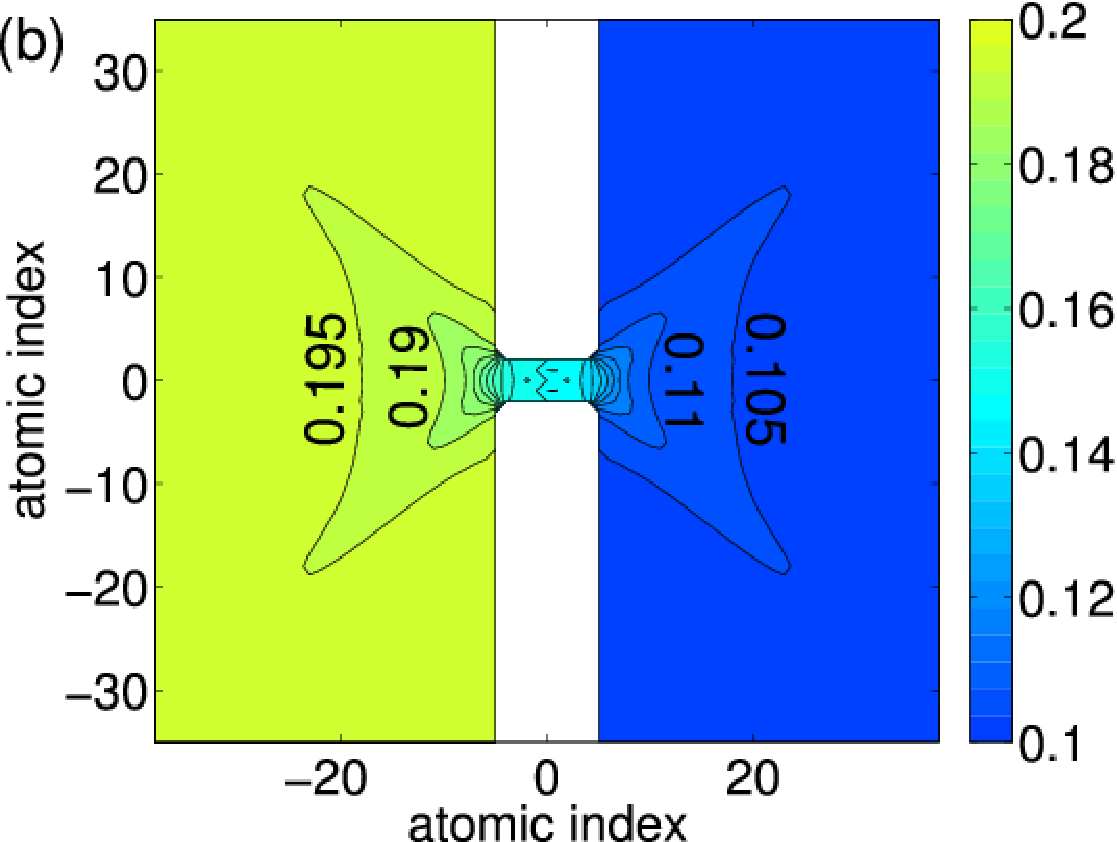
\includegraphics[width=.49\columnwidth]{pics/gf_fig7b.pdf}
 \caption{Bath temperature profiles in a $w=5$, $l=9$ constriction coupled to leads of width $W=71$ and $L=35$ [see Fig. \ref{fig:chain_rg}(b)]. Lead temperatures are $T_L=0.2$ and $T_R=0.1$. Figures show (a) quantum exact and (b) classical self-consistent bath temperature profiles. Friction parameter is $\gamma=0.01$. The separation of isolines is $0.05$ and four contour lines are labeled for convenience.}
 \label{fig:gf_fig7}
\end{figure}

\begin{figure}
 \begin{center}
 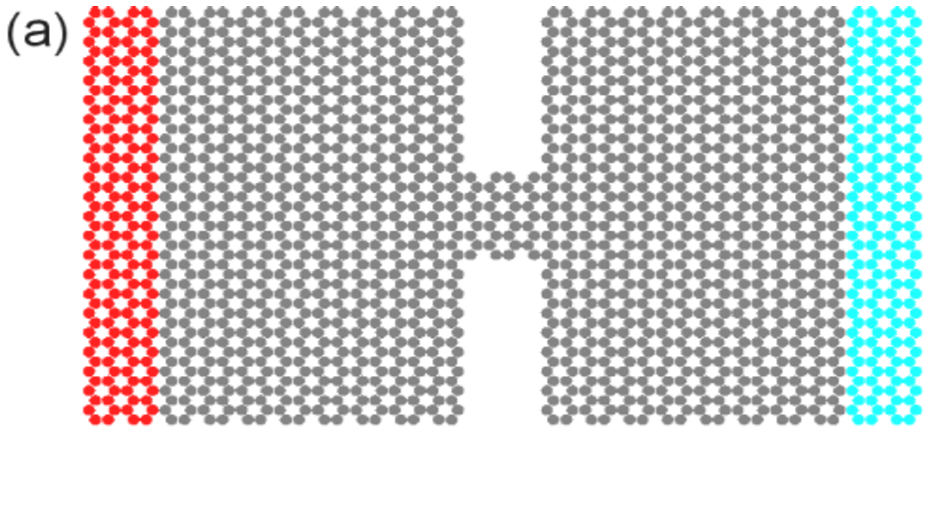
\includegraphics[width=.49\columnwidth]{pics/gf_fig8a.pdf}
 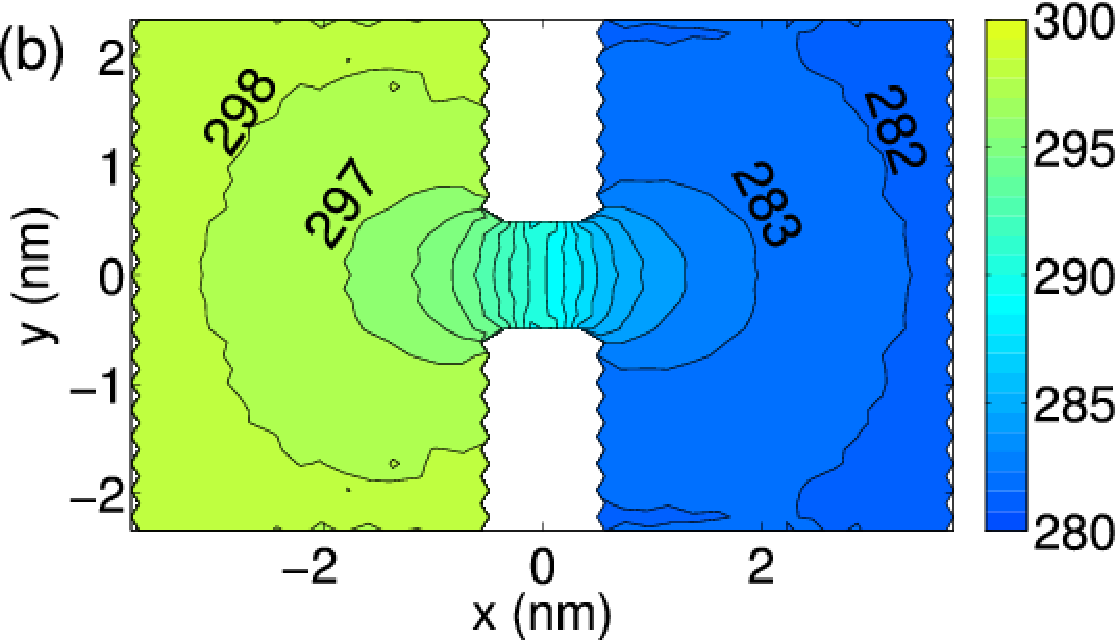
\includegraphics[width=.49\columnwidth]{pics/gf_fig8b.pdf}
 \end{center}
 \caption{(a) Graphene nanoconstriction. The leads extend infinitely to the left and right, but the temperatures are determined self-consistently only for the gray atoms in the shown center region. (b) Self-consistent bath temperature profiles (K). The semi-infinite leads are at temperatures $T_L=300$ K and $T_R=280$ K. The relaxation time $\tau=1/\gamma$ is set to $1$ ps.}
 \label{fig:gf_fig8}
\end{figure}

\subsection{Anharmonic effects at interfaces (\cp{spectral})}

\begin{figure}[tb]
 \begin{center}
  %\includegraphics[width=.99\columnwidth]{/Users/saaskilak/Documents/matlab/pics/171213a_cnt.ps}
 % \includegraphics[width=.99\columnwidth]{/Users/saaskilak/Documents/latex/pics/240114_fcc_final.ps}
  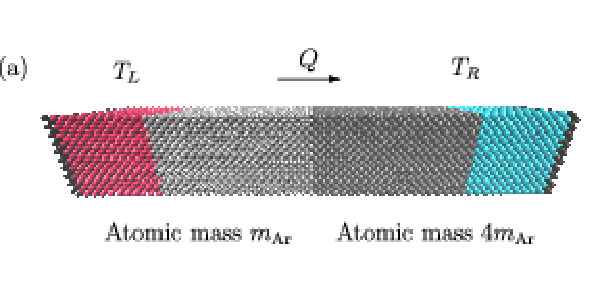
\includegraphics[width=8.6cm]{pics/nemd_fig2a.pdf}
  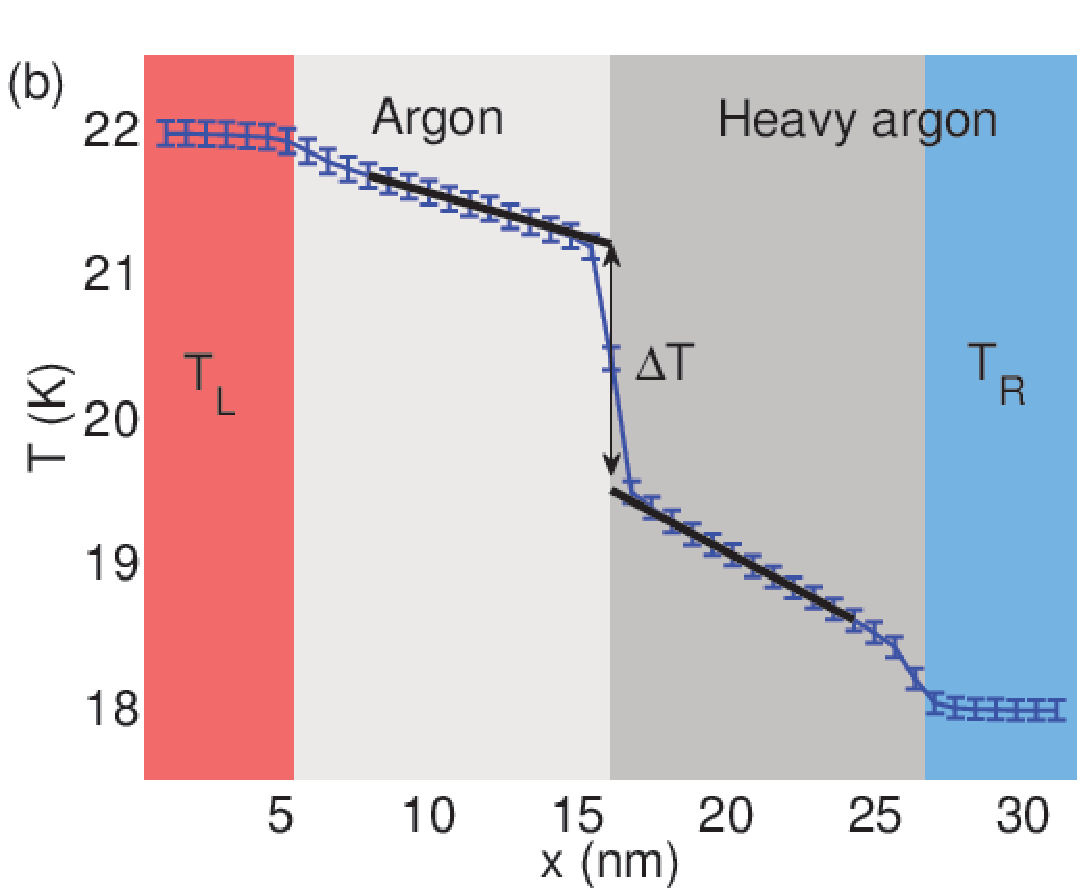
\includegraphics[width=8.6cm]{pics/nemd_fig2b.pdf}
  \caption{(a) Atomistic illustration of the studied interface between two mass-mismatched Lennard-Jones solids. The atoms at the left and right ends are coupled to Langevin heat baths at different temperatures $T_L$ and $T_R$ to drive thermal current $Q$ through the interface in the middle. (b) Local kinetic temperature profile in a non-equilibrium simulation with average temperature $T=20$ K. Temperature drop $\Delta T$ at the interface is estimated by extrapolating the linear fits to the temperature profiles at different sides of the interface and calculating the difference at the interface. } 
 \label{fig:nemd_fig2}
 \end{center}
\end{figure}

\begin{figure}[tb]
 \begin{center}
  %\includegraphics[width=.99\columnwidth]{/Users/saaskilak/Documents/matlab/pics/171213a_cnt.ps}
 % \includegraphics[width=.99\columnwidth]{/Users/saaskilak/Documents/latex/pics/240114_fcc_final.ps}
  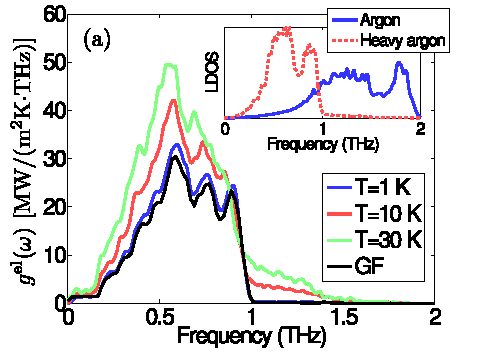
\includegraphics[width=.49\columnwidth]{pics/nemd_fig4a.pdf}
  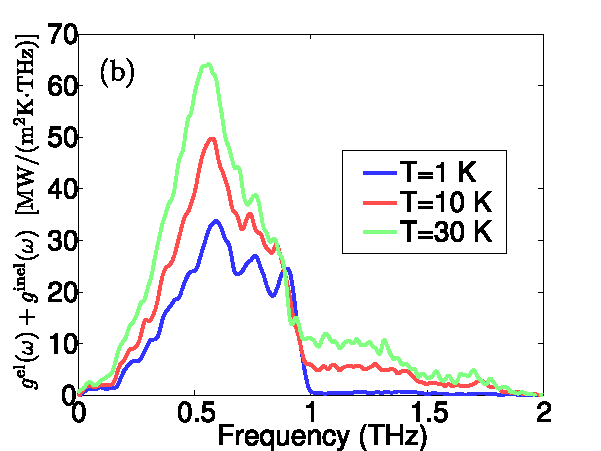
\includegraphics[width=.49\columnwidth]{pics/nemd_fig4b.pdf}
  \caption{The elastic conductance  \eqref{eq:gel} as a function of frequency at various temperatures. At $T=1$ K, the elastic conductance agrees very well with the Landauer-B\"uttiker conductance $g^{\textrm{LB}} (\omega)=k_B \mathcal{T}(\omega)/A$, where the transmission function $\mathcal{T}(\omega)$ has been calculated for the interface between two semi-infinite LJ solids using the Green's function (GF) method. At high temperatures, inelastic effects in the bulk enable energy transmission also above the cut-off frequency $f_c^{(2)}=1$ THz of the heavier solid. Inset: Local density of vibrational states (LDOS, arbitrary units) at the interface calculated from MD at $T=1$ K. In the lighter solid with mass $m_1=m_{\textrm{Ar}}$ (argon, solid line), vibration frequency cut-off is $f_c^{(1)}=2$ THz. In the heavier medium with mass $m_2=4m_1$ (heavy argon, dashed line), bulk vibrations therefore only extend up to $f_c^{(2)}=1$ THz, limiting ballistic transmission of phonons below this limit. At the interface, however, there are evanescent wave states extending up to 1.5 THz. (b) The sum $g^{\textrm{el}}(\omega)+ g^{\textrm{inel}}(\omega)$ of elastic and inelastic [Eq. \eqref{eq:ginel_dec}] spectral conductance as a function of frequency. At high temperatures, the inelastic energy transfer processes strongly enhance interfacial heat transfer at $f\approx 0.5$ THz and above the cut-off $f_c^{(2)}=1$ THz.} 
 \label{fig:nemd_fig2}
 \end{center}
\end{figure}

\begin{figure}[tb]
 \begin{center}
  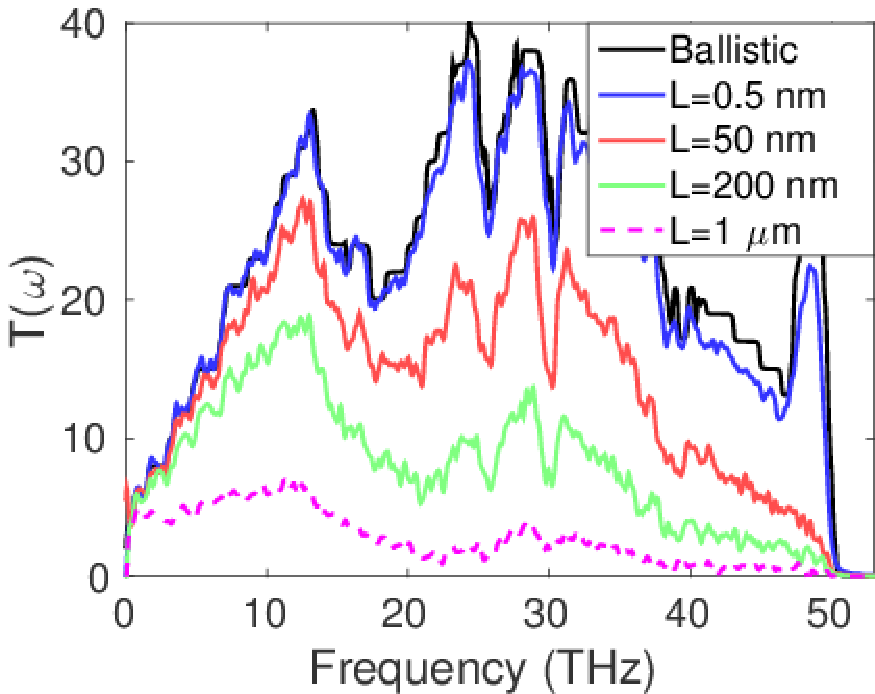
\includegraphics[width=.49\columnwidth]{pics/cnt_fig2.pdf} 
  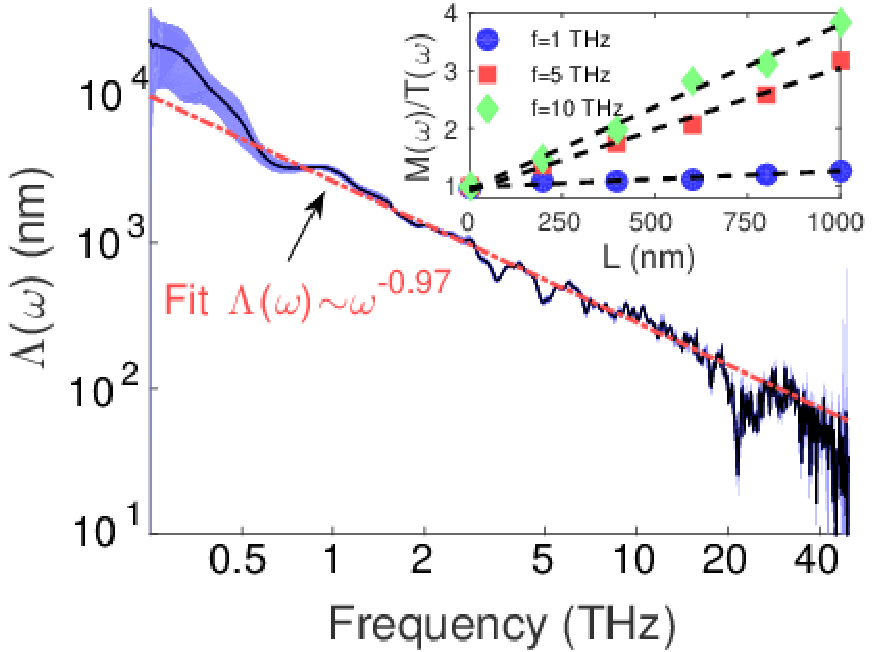
\includegraphics[width=.49\columnwidth]{pics/cnt_fig4.pdf} 
  \caption{(a) Spectral transmission function $\ca{T}(\omega)=q(\omega)/(k_B\Delta T)$ for various tube lengths at $T=300$ K, determined from the NEMD simulations. As expected, increasing the tube length reduces the transmission. For $L=0.5$ nm, the spectral conductance is very close to the ballistic value $M(\omega)$ determined by counting the number of propagating modes from the phonon bandstructure of Fig. \ref{fig:bs}. (b) Log-log plot of the mean free path $\Lambda(\omega)$ at $T=300$ K. The inset shows the scaled inverse transmission functions $M(\omega)/\ca{T}(\omega)$ as a function of tube length $L$. The mean free paths are determined from the inverse slopes of the least-square linear fits (dashed, black lines in the inset) calculated using an automated numerical routine at each frequency. The shaded regions in the main figure correspond to the 92.5\% confidence interval for the slope. Below 0.25 THz, the confidence interval is very large (not shown) due to numerical uncertainties, inhibiting the reliable determination of mean free paths for very small frequencies.}  
\label{fig:cnt_fig2}
 \end{center}
\end{figure}

\begin{figure}[tb]
 \begin{center}
  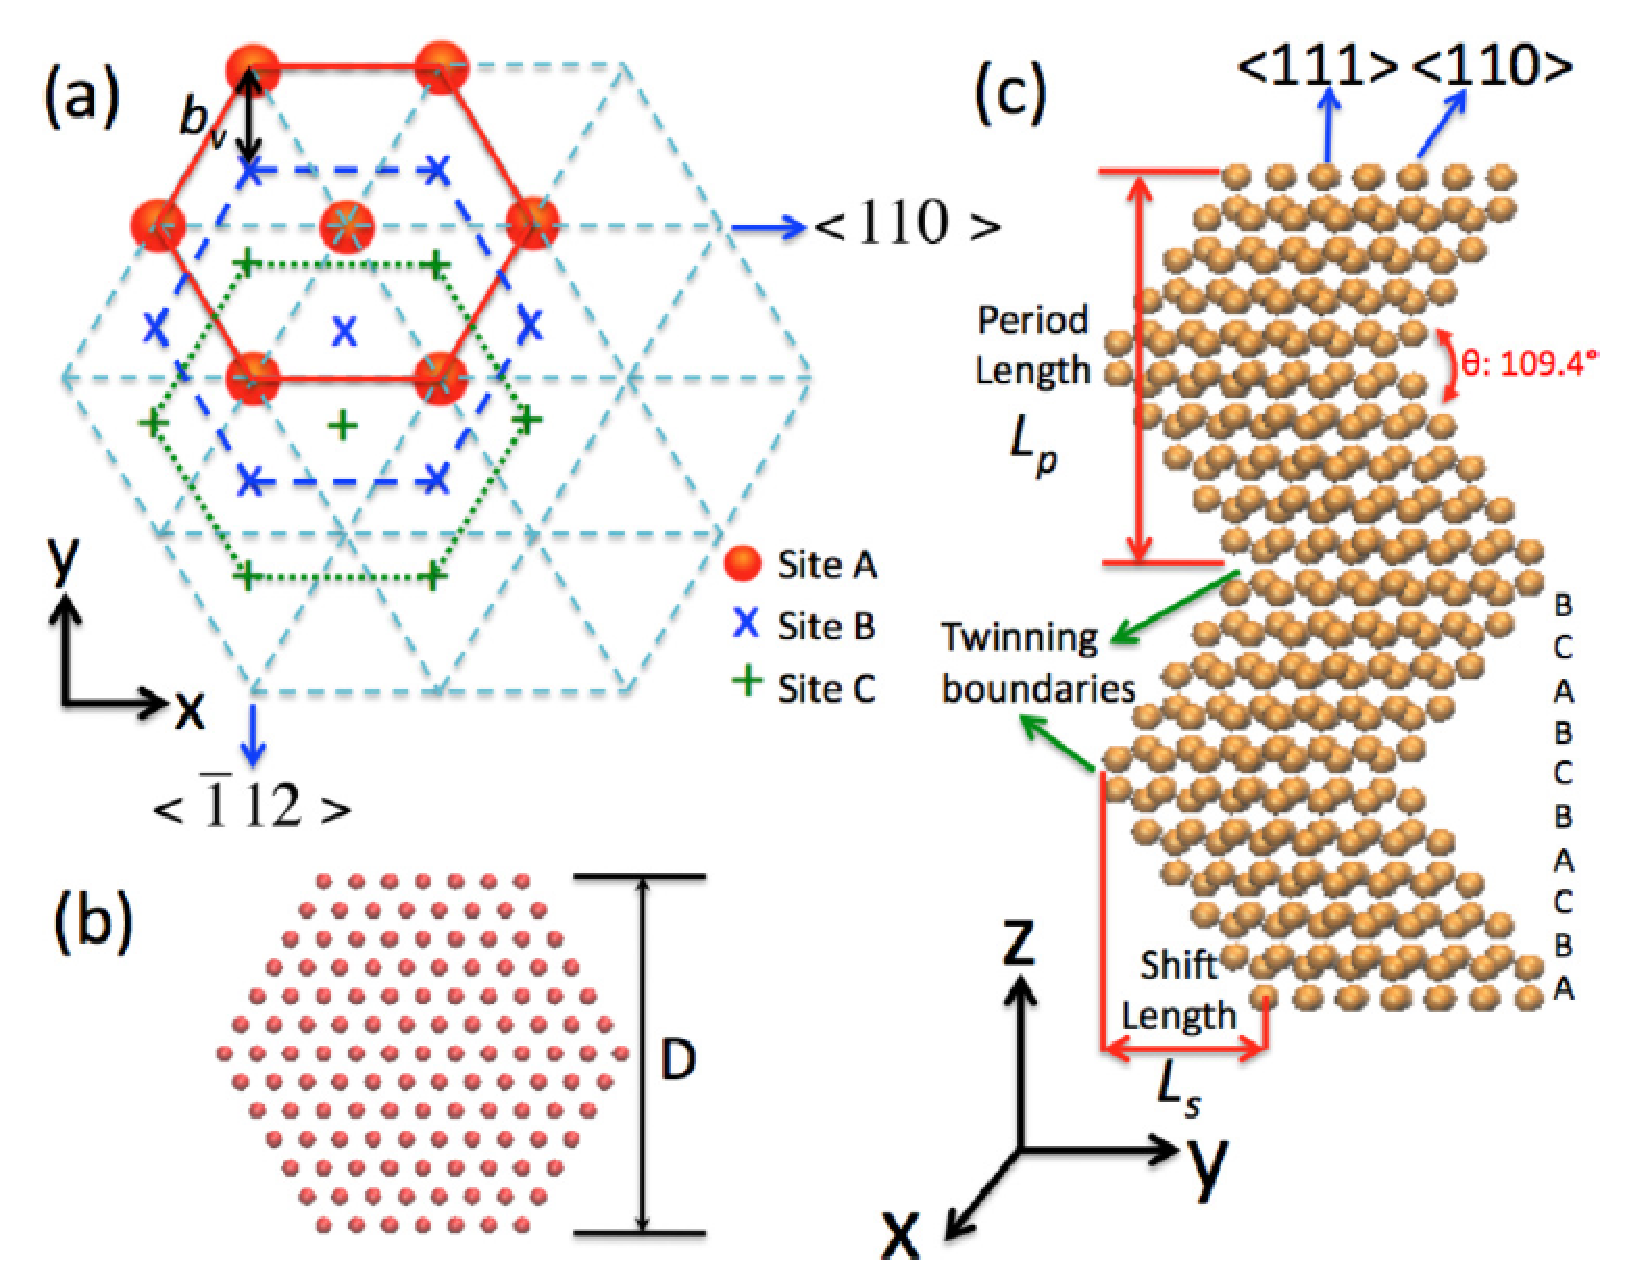
\includegraphics[width=.49\columnwidth]{pics/twinning_fig1.pdf} 
  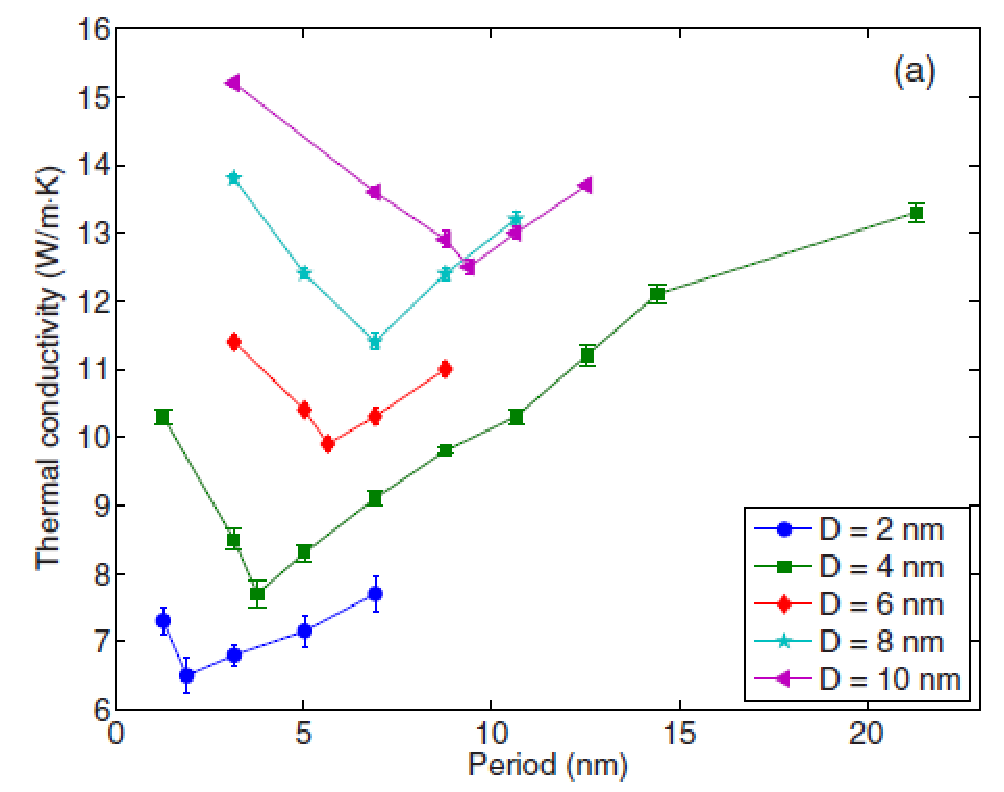
\includegraphics[width=.49\columnwidth]{pics/twinning_fig2a.pdf} 
  \caption{}  
\label{fig:twinning_fig1}
 \end{center}
\end{figure}

\subsection{Mean free paths in carbon nanotubes (\cp{cnt})}

\subsection{Minimum thermal conductivity in twinning Si nanowires (\cp{twinning})}
